\documentclass[11pt]{article}

\usepackage[margin=1in]{geometry}
\usepackage[T1]{fontenc}
\usepackage{lmodern}
\usepackage{microtype}
\usepackage{amsmath, amssymb}
\usepackage{booktabs}
\usepackage{array}
\usepackage{tabularx}
\usepackage{tikz}
\usetikzlibrary{arrows.meta, positioning, shapes.geometric, calc, decorations.pathreplacing, backgrounds}
\usepackage{float}
\usepackage[hidelinks]{hyperref}
\usepackage{caption}
\usepackage{xcolor}
\usepackage{enumitem}
\usepackage[round]{natbib}

\setlength{\parskip}{0.5em}
\setlength{\parindent}{0pt}

\newcommand{\predstart}{\text{pred\_start}}
\newcommand{\predstop}{\text{pred\_stop}}

\title{\textbf{FLAIR Task Schematic} \\[0.3em]
       ICU Daily LTACH Discharge at 07:00 Local (Task T2)}
\author{FLAIR Benchmark}
\date{\today}

\begin{document}
\maketitle

\begin{abstract}
\noindent We specify the FLAIR daily ICU LTACH-discharge task: at
every local 07:00 rounds anchor during the first ICU stay, predict
whether the hospitalization will end with transfer to a Long-Term
Acute Care Hospital (CLIF \texttt{discharge\_category} $=$
\texttt{Long Term Care Hospital (LTACH)}). The cohort is identical
to Task~T1 (all adult ICU hospitalizations, no
\texttt{discharge\_category} filter); only the label predicate
differs. T1 and T2 are \textbf{not} a partition: a stay discharged
Home is label-0 in both; a stay discharged Expired is label-1 in T1
and label-0 in T2. The shared pipeline is specified once in
\texttt{icu\_daily\_mortality.tex} (Task~T1); this schematic specifies
only the T2 label rule and its design rationale.
\end{abstract}

\section{Relationship to Task~T1}

The build pipeline of Task~T2 is byte-identical to Task~T1's: same
cohort filters (adult, valid admission/discharge, $\geq 1$ ICU ADT
record, first ICU stay long enough for at least one 07:00 grid point),
same $\predstart$, $\predstop$, and decision-point grid, same 24h
lookback, same temporal split. \textbf{Neither task filters on
\texttt{discharge\_category} at the cohort stage.} The only difference
is the final label rule. The full operational definition, cohort
details, and step-by-step build logic are in
\texttt{icu\_daily\_mortality.tex} (Task~T1); the flowchart of
Figure~\ref{fig:t2-flow} is shared.

\section{Label rule (Task~T2 only)}

Let
$\texttt{disp}_i = \texttt{lower}(\texttt{strip}(\texttt{discharge\_category}_i))$.
For $d$ in the daily 07:00 decision grid $D_i$:
\[
y_i(d) \;=\; \mathbb{1}\!\left[\,\texttt{disp}_i\ \text{matches regex}\
\texttt{ltach|long.?term}\,\right].
\]

\begin{itemize}[leftmargin=2em]
  \item The label is constant across all rows of $H_i$ (the eventual
        disposition is a single hospitalization-level fact broadcast
        to every grid point).
  \item A null \texttt{disp}$_i$ (i.e., \texttt{discharge\_category}
        null in the source) or any non-matching value
        (\texttt{Expired}, \texttt{Hospice}, \texttt{Home},
        \texttt{Skilled Nursing Facility (SNF)},
        \texttt{Acute Inpatient Rehab Facility},
        \texttt{Against Medical Advice (AMA)}, \texttt{Other},
        \texttt{Still Admitted}, \ldots) yields $y_i(d) = 0$.
  \item Because Tasks~T1 and T2 share the same unconditional cohort
        and have non-overlapping label predicates,
        $\texttt{label\_mortality}_i + \texttt{label\_ltach}_i \le 1$
        but \textbf{not} necessarily $= 1$: a Home discharge is 0 in
        both, an Expired discharge is 1 in T1 / 0 in T2, and an
        LTACH discharge is 0 in T1 / 1 in T2.
\end{itemize}

\section{CLIF tables and categories used}

The CLIF surface for Task~T2 is identical to Task~T1: the same three
tables (\texttt{hospitalization}, \texttt{patient}, \texttt{adt}) and
the same cohort filters. The ADT filter restricts to
\texttt{location\_category} $=$ \texttt{"icu"} (case-insensitive);
\texttt{patient} is join-only; \texttt{discharge\_category} is read
from \texttt{hospitalization} for the \emph{label} only --- no cohort
filter is applied on it. See the full table and per-table column
inventory in the sibling document \texttt{icu\_daily\_mortality.tex}
(\S CLIF tables and categories used). Tasks~T1 and~T2 differ only in
the final label predicate, not in which CLIF data they touch.

\section{Algorithmic flow (shared with Task~T1)}

\begin{figure}[H]
\centering
% Algorithmic flowchart for FLAIR ICU daily disposition tasks (T1 mortality / T2 LTACH).
% Both tasks share an unconditional cohort and pipeline; only the final label rule differs.

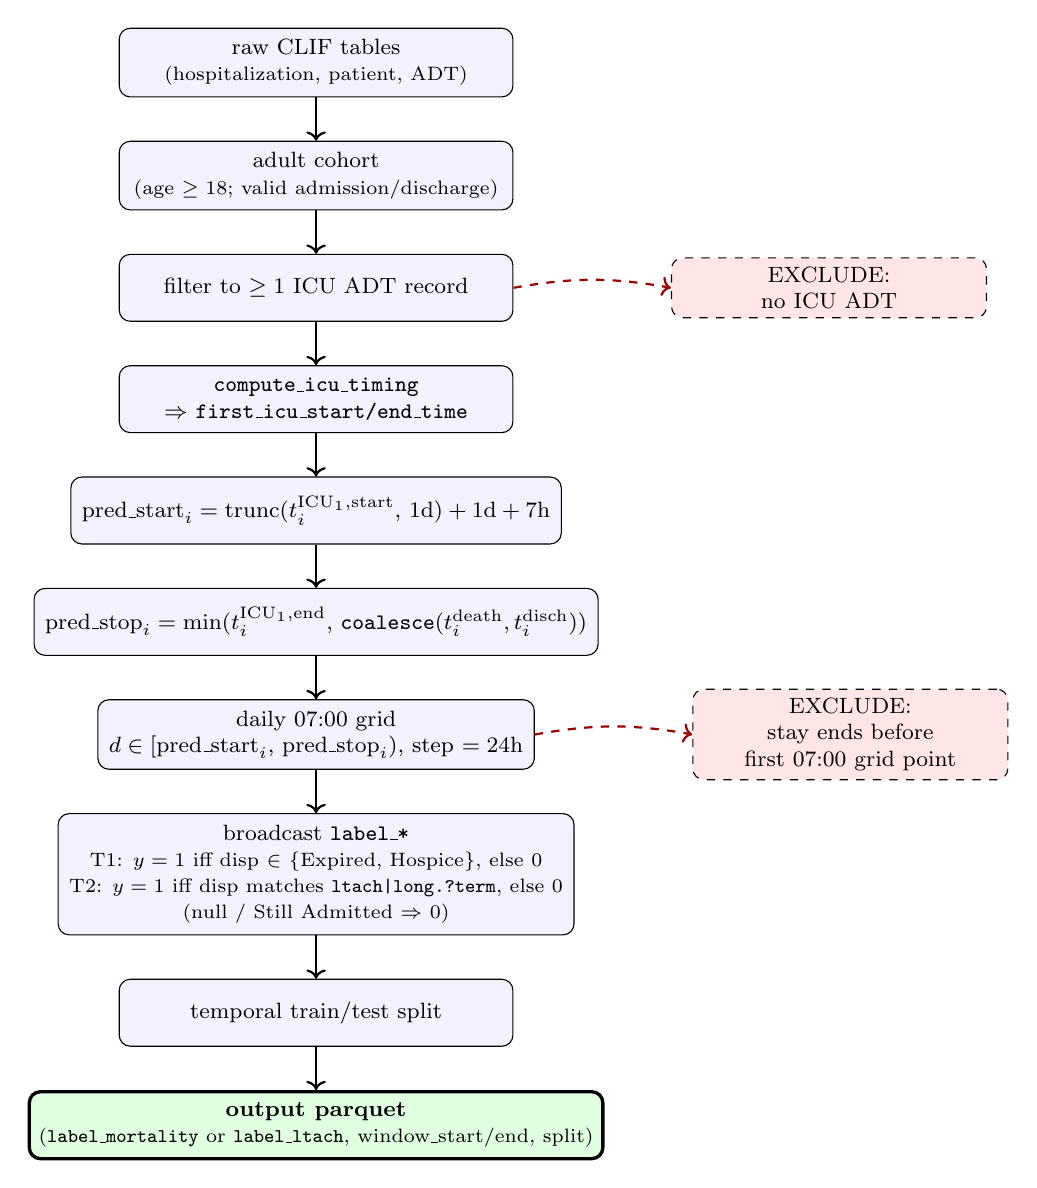
\begin{tikzpicture}[
    node distance=0.55cm and 0.7cm,
    every node/.style={font=\footnotesize, align=center},
    box/.style={draw, rounded corners, fill=blue!5,
                minimum width=5.0cm, minimum height=0.85cm, inner sep=4pt},
    excl/.style={draw, rounded corners, fill=red!10, dashed,
                 minimum width=4.0cm, minimum height=0.7cm},
    outbox/.style={draw, rounded corners, fill=green!12, very thick,
                minimum width=5.0cm, minimum height=0.85cm},
    arrow/.style={->, thick},
    sidearrow/.style={->, thick, red!60!black, dashed},
]
    % main pipeline
    \node[box] (raw)
        {raw CLIF tables\\\scriptsize(hospitalization, patient, ADT)};
    \node[box, below=of raw] (cohort)
        {adult cohort\\\scriptsize(age $\geq 18$; valid admission/discharge)};
    \node[box, below=of cohort] (icu)
        {filter to $\geq 1$ ICU ADT record};
    \node[box, below=of icu] (timing)
        {\texttt{compute\_icu\_timing}\\$\Rightarrow$ \texttt{first\_icu\_start/end\_time}};
    \node[box, below=of timing] (predstart)
        {$\predstart_i = \text{trunc}(t^{\text{ICU}_1,\text{start}}_i,\,1\text{d})
         + 1\text{d} + 7\text{h}$};
    \node[box, below=of predstart] (predstop)
        {$\predstop_i = \min(t^{\text{ICU}_1,\text{end}}_i,\,
         \texttt{coalesce}(t^{\text{death}}_i, t^{\text{disch}}_i))$};
    \node[box, below=of predstop] (grid)
        {daily 07:00 grid\\$d \in [\predstart_i,\, \predstop_i)$, step $= 24$h};
    \node[box, below=of grid] (label)
        {broadcast \texttt{label\_*}\\\scriptsize{T1: $y = 1$ iff disp $\in$
         \{Expired, Hospice\}, else 0}\\\scriptsize{T2: $y = 1$ iff disp matches
         \texttt{ltach|long.?term}, else 0}\\\scriptsize{(null / Still Admitted $\Rightarrow$ 0)}};
    \node[box, below=of label] (split)
        {temporal train/test split};
    \node[outbox, below=of split] (parquet)
        {\textbf{output parquet}\\\scriptsize{(\texttt{label\_mortality} or
         \texttt{label\_ltach}, window\_start/end, split)}};

    % exclusions on the right
    \node[excl, right=2.0cm of icu] (exclNoIcu)
        {EXCLUDE:\\no ICU ADT};
    \node[excl, right=2.0cm of grid] (exclShort)
        {EXCLUDE:\\stay ends before\\first 07:00 grid point};

    % main arrows
    \draw[arrow] (raw) -- (cohort);
    \draw[arrow] (cohort) -- (icu);
    \draw[arrow] (icu) -- (timing);
    \draw[arrow] (timing) -- (predstart);
    \draw[arrow] (predstart) -- (predstop);
    \draw[arrow] (predstop) -- (grid);
    \draw[arrow] (grid) -- (label);
    \draw[arrow] (label) -- (split);
    \draw[arrow] (split) -- (parquet);

    % exclusion arrows
    \draw[sidearrow] (icu.east) to[bend left=10] (exclNoIcu.west);
    \draw[sidearrow] (grid.east) to[bend left=10] (exclShort.west);

\end{tikzpicture}

\caption{Build pipeline shared by Tasks~T1 and T2. The label box at
the bottom is parameterized: T2 emits $y = 1$ iff
\texttt{disp}\textsubscript{i} matches \texttt{ltach|long.?term}.
Everything else --- cohort filters, ICU timing, $\predstart$ /
$\predstop$, the daily 07:00 grid, the 24h lookback, the temporal
split, the parquet schema --- is identical to Task~T1.}
\label{fig:t2-flow}
\end{figure}

\section{Design choices and rationale}

\paragraph{Why a separate schematic for a different label on the same cohort.}
A reader scanning the supplement should find one document per FLAIR
task, with its own META, label rule, and prevalence numbers. The
build pipeline being shared is a convenience of implementation, not a
property of the task definition: a future site whose
\texttt{discharge\_category} taxonomy splits LTACH from other
long-term destinations more finely could change Task~T2's regex
without affecting Task~T1.

\paragraph{Prevalence and class imbalance.}
LTACH transfer is a rare disposition in the absolute sense: across
all adult ICU stays it sits in the low single digits per-row positive
rate. Class imbalance is therefore the dominant modelling challenge,
and AUPRC is the primary headline metric. AUROC is reported but is
known to be optimistic on heavily imbalanced binary tasks.

\paragraph{Why LTACH is the operationally interesting label.}
LTACH transfer is a planned, resource-intensive disposition decision
that triggers care-coordination work several days before discharge
\citep{kahn2010ltach}. A morning prediction of LTACH-bound trajectory
can drive social-work referrals, family conversations, and
family-meeting timing.

\paragraph{Why an unconditional cohort.}
Earlier drafts conditioned the cohort on the union of LTACH and
in-hospital mortality, manufacturing a balanced binary against T1.
That design has been retired (see Task~T1 schematic, \S Design
choices). The unconditional cohort makes the per-row positive rate
interpretable as the prevalence of LTACH-bound trajectories among all
ICU survivors-and-non-survivors, and matches the standard
ICU-outcome-prediction setup.

\section{Out of scope}

\begin{itemize}[leftmargin=2em]
  \item All items listed in \texttt{icu\_daily\_mortality.tex}
        (Task~T1) \S\textit{Out of scope} carry over.
  \item Finer-grained LTACH-vs-skilled-long-term-care distinctions
        within the LTACH-positive class.
\end{itemize}

\bibliographystyle{plainnat}
\bibliography{references}

\end{document}
